% Starting point for drawing neural networks.
% Not finished.
% Original source code: http://www.texample.net/tikz/examples/neural-network/
\def\layersep{2.5cm}

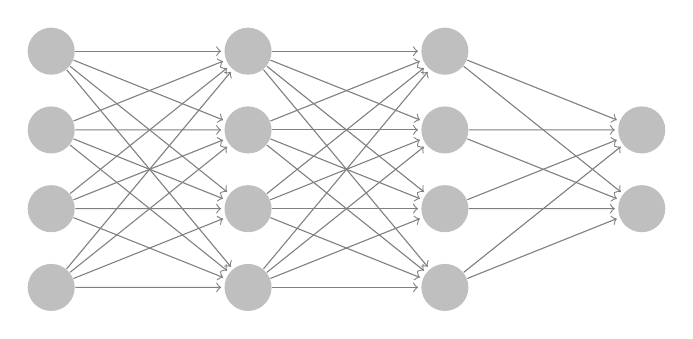
\begin{tikzpicture}[shorten >=1pt,->,draw=black!50, node distance=\layersep]
    \tikzstyle{every pin edge}=[<-,shorten <=1pt]
    \tikzstyle{neuron}=[circle,fill=black!25,minimum size=17pt,inner sep=0pt]

    \foreach \name / \y in {1,...,4}
        \node[neuron] (I-\name) at (0,-\y) {};

    \foreach \name / \y in {1,...,4}
        \path node[neuron] (H-\name) at (\layersep,-\y cm) {};

    \foreach \name / \y in {1,...,4}
        \path node[neuron] (O-\name) at (2*\layersep,-\y cm) {};

    \foreach \name / \y in {1,...,2}
        \path node[neuron, yshift=-1cm] (F-\name) at (3*\layersep,-\y cm) {};

    \foreach \source in {1,...,4}
        \foreach \dest in {1,...,4}
            \path (I-\source) edge (H-\dest);

    \foreach \source in {1,...,4}
        \foreach \dest in {1,...,4}
            \path (H-\source) edge (O-\dest);

    \foreach \source in {1,...,4}
        \foreach \dest in {1,...,2}
            \path (O-\source) edge (F-\dest);

    \begin{scope}[xshift=3*\layersep]
    \end{scope}
\end{tikzpicture}
